\newpage
\section{Theoretical Analysis}
\label{sec:analysis}

\subsection{Exercise 1}
\label{Exercise 1}

%---------------Theoretical Analysis Exercise 1--------------------------------------------------------%
\begin{figure}[!ht] \centering
\caption{Representation of mesh currents in the circuit.}
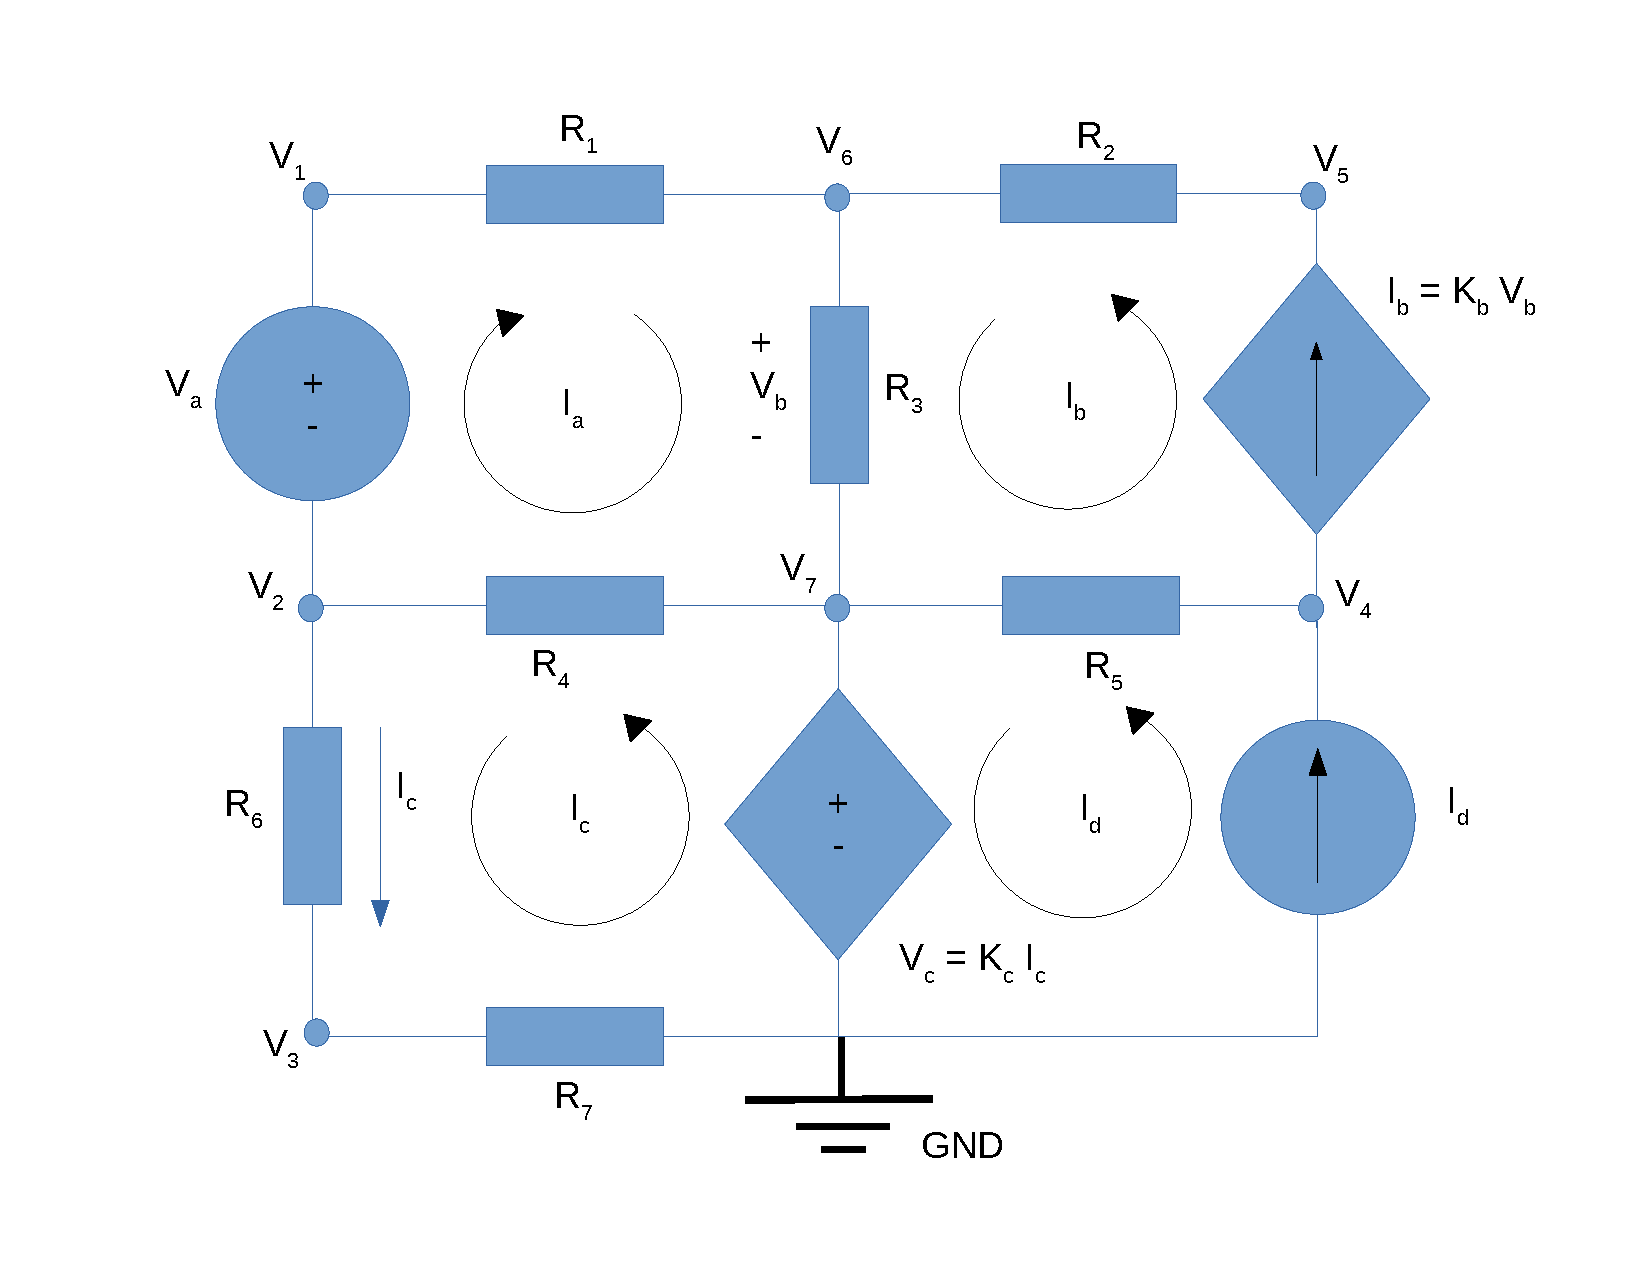
\includegraphics[width=0.8\linewidth]{circuit_mesh.pdf}
\label{fig:meshcurrents}
\end{figure}

Figure~\ref{fig:meshcurrents} shows the mesh currents considered for the circuit analysis, with the current $I_a$ flowing clockwise and the rest of the currents ($I_b$, $I_c$ and $I_d$) flowing counter-clockwise. In the meshes containing $I_b$ and $I_d$, the currents were considered to be the same as the current sources in said meshes.

From this circuit, there can then be extracted 3 equations to figure out the value of the components necessary for the circuit analysis.

The first one, Equation~\ref{eq:meshb}, was obtained by using Ohm's Law, assuming it is known the value of the voltage and the resistance in resistor 3 and that the current flowing through it is ($I_a$ + $I_b$).
\begin{equation}
  I_{b} = K_{b}(I_{a} + I_{b})R_{3},
  \label{eq:meshb}
\end{equation}

Equation~\ref{eq:mesha}  was figured out by analysing the top left mesh, using Kirchoff's Voltage Law and Ohm's Law for the resistors. Since the current $I_a$ is flowing clockwise, the voltage in $V_a$ is negative and the currents in resistors 3 and 4 are, 
correspondingly, ($I_a$ + $I_b$) and ($I_a$ + $I_c$), as these pairs of currents are flowing the same way in said resistors.
\begin{equation}
  -V_{a} + I_{a}R_{1} + (I_{a} + I_{b})R_{3} + (I_{a} + I_{c})R_{4} = 0,
  \label{eq:mesha}
\end{equation}

Finally, from the bottom left mesh, there is Equation~\ref{eq:meshc}, in which was also used Kirchoff's Voltage Law and Ohm's Law. The voltage in $V_c$ is negative due to the current flow.
\begin{equation}
  -K_{c}I_{c} + I_{c}R_{6} + I_{c}R_{7} + (I_{a} + I_{c})R_{4} = 0,
  \label{eq:meshc}
\end{equation}
\newpage

By developing these 3 equations, the matrix below (\ref{eq:matrix}) is achieved as to simplify the calculations. This matrix was solved in Octave, getting the values of the currents $I_a$, $I_b$ and $I_c$ that can be found in table~\ref{table:nodesmesh}. It was not necessary to solve for the value of the current in the bottom right mesh since it is already known (equivalent to $I_d$).

\begin{equation}
\left[ \begin{array}{ccc} -K_bR_3 & 1-K_bR_3 & 0 \\ R_1+R_3+R_4 & R_3 & R_4 \\ R_4 & 0 & R_6+R_7-K_c+R_4 \end{array} \right]
\times \left[ \begin{array}{c} I_a \\ I_b \\ I_c \end{array} \right] =
\left[ \begin{array}{c} 0 \\ V_a \\ 0 \end{array} \right]
\label{eq:matrix}
\end{equation}

With these currents, it is possible to discover the values of the voltages in each node, using the equations~\ref{eq:node7} through~\ref{eq:node1} down below and knowing that $I_b$ = $K_b$$V_b$ and $V_c$=$K_c$$I_c$.
\begin{equation}
  V_{7} = V_{c},
  \label{eq:node7}
\end{equation}

\begin{equation}
  V_{6} = V_{7} + V_{b},
  \label{eq:node6}
\end{equation}

\begin{equation}
  V_{5} = V_{6} + R_{2}I_{b},
  \label{eq:node5}
\end{equation}

\begin{equation}
  V_{4} = V_{7} + R_{5}(I_{d} - I_{b}),
  \label{eq:node4}
\end{equation}

\begin{equation}
  V_{3} = V_{0} + R_{7}I_{c},
  \label{eq:node3}
\end{equation}

\begin{equation}
  V_{2} = V_{3} + R_{6}I_{c},
  \label{eq:node2}
\end{equation}

\begin{equation}
  V_{1} = V_{2} + V_{a},
  \label{eq:node1}
\end{equation}

Table~\ref{table:theoretical_1} shows the nodes' voltages discovered by replacing the known variables in equations~\ref{eq:node7} to ~\ref{eq:node1}. The branch currents were obtained with the following equations~\ref{eq:branch1} to ~\ref{eq:branch6/7} (resorting to figure~\ref{fig:meshcurrents}).

\begin{equation}
  R_1[i] = I_a,
  \label{eq:branch1}
\end{equation}

\begin{equation}
  R_2[i]= I_b,
  \label{eq:branch2}
\end{equation}

\begin{equation}
  R_3[i] = I_a + I_b,
  \label{eq:branch3}
\end{equation}

\begin{equation}
  R_4[i] = I_a + I_c,
  \label{eq:branch4}
\end{equation}

\begin{equation}
  R_5[i] = Id - Ib,
  \label{eq:branch5}
\end{equation}

\begin{equation}
  R_6[i] = R_7[i] = I_c,
  \label{eq:branch6/7}
\end{equation}



\begin{table}[!ht]
\centering
\begin{tabular}{ |c|c|} 
 \hline
 {\bf Node} & {\bf Voltage[V]} \\ 
 \hline\hline
  $V_b$ & \partialinput{1}{1}{theoretical_1.tex}\\ 
 \hline
  $V_d$ & \partialinput{2}{2}{theoretical_1.tex} \\ 
 \hline
 $V_1$ & \partialinput{3}{3}{theoretical_1.tex} \\ 
 \hline
 $V_2$ & \partialinput{4}{4}{theoretical_1.tex} \\ 
 \hline
 $V_3$ & \partialinput{5}{5}{theoretical_1.tex} \\ 
 \hline
 $V_5$ & \partialinput{6}{6}{theoretical_1.tex} \\ 
 \hline
 $V_6$ & \partialinput{7}{7}{theoretical_1.tex} \\ 
\hline
 $V_6$ & \partialinput{8}{8}{theoretical_1.tex} \\ 
 \hline
 $V_8$ & \partialinput{9}{9}{theoretical_1.tex} \\
 \hline
\end{tabular}
\begin{tabular}{ |c|c|} 
 \hline
 {\bf Branch} & {\bf Current[A]}\\ 
 \hline\hline
 $I_b$ & \partialinput{10}{10}{theoretical_1.tex} \\ 
 \hline
 $I_c$ & \partialinput{11}{11}{theoretical_1.tex} \\
 \hline
 $I_d$ & \partialinput{12}{12}{theoretical_1.tex} \\
 \hline
 %$R_1=I_a$ & \partialinput{12}{12}{malhas.tex} \\ 
 %\hline
 % $R_2$ & \partialinput{13}{13}{malhas.tex} \\ 
 %\hline
 % $R_3$ & \partialinput{14}{14}{malhas.tex} \\  
 %\hline
 %$R_4$ & \partialinput{15}{15}{malhas.tex} \\ 
 %\hline
 %$R_5$ & \partialinput{16}{16}{malhas.tex} \\  
 %\hline
 %$R_6$ & \partialinput{17}{17}{malhas.tex} \\ 
 %\hline
 % $R_7$ & \partialinput{18}{18}{malhas.tex} \\  
 %\hline
\end{tabular}
\caption{Voltage and Current values(Exercise 1)}
\label{table:theoretical_1}
\end{table}

\begin{figure}[!ht] \centering
\caption{Final solution of $v_6(t)$ and $v_s(t)$ in the interval $[-5,20]ms$}
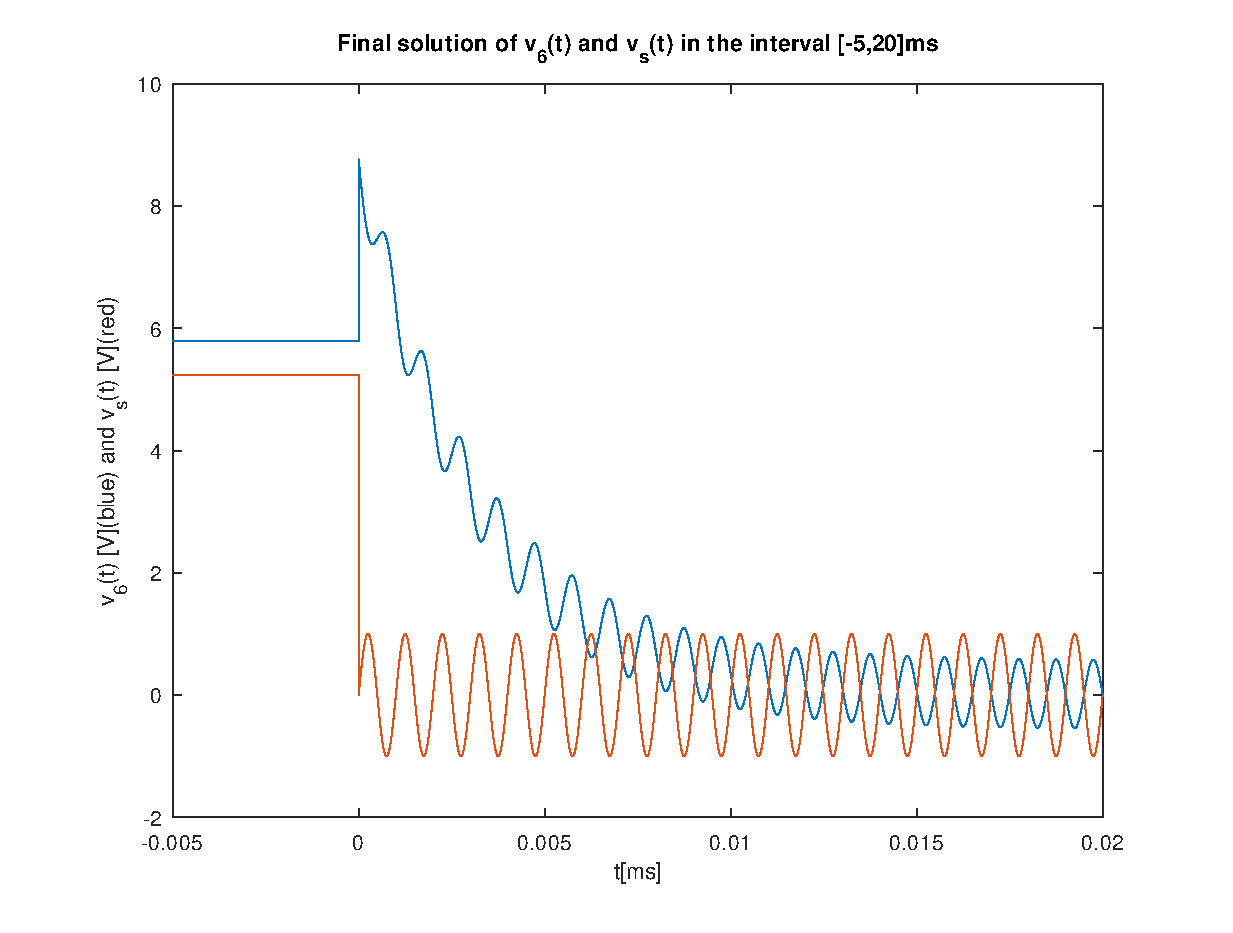
\includegraphics[width=0.8\linewidth]{theoretical_5.eps}
\label{fig:circuit}
\end{figure}






